% !TeX root=../main.tex
\chapter{مدل کردن مدار به صورت گراف}
%\thispagestyle{empty} 
\label{chap:results}
\section{پیشگفتار} 
در دو فصل پیش بر آنچه که برای مدل کردن مدار های الکتریکی به صورت گراف نیاز داریم
مرور کوتاهی شد؛ در این فصل با در آمیختن این دانش ها تلاش میشود مدار را به صورت ریاضی مدل کرده
و به صورت خودکار پاسخ آن را پیدا کنیم.
\section{گراف کیرشهف}
با در نظر گرفتن گره های مدار به عنوان راس های گراف، و شاخه های مدار به عنوان یال های گراف
میتوانیم مدار را به صورت یک گراف مدل کنیم.
در این مدل اجزای الکتریکی مدار به عنوان 
\lr{edge attribute}
در نظر گرفته میشوند.

پس از مدل کردن مدار به صورت گراف، قوانین جریان و ولتاژ کیرشهف را اعمال میکنیم تا به یک
معادله ماتریسی
\footnote{
	این معادله ماتریسی در مورد مدار های دارای خازن و سلف یک معادله دیفرانسیل ماتریسی است
	در غیر این صورت یک معادله جبری ماتریسی است.
}
برسیم حل این معادله ماتریسی جریان هر شاخه مدار را به ما خواهد داد.

در ادامه با حل چندین نمونه سعی در روشنتر شدن موضوع میکنیم.

\section{حل یک نمونه از مدار های بدون خازن و سلف}
به عنوان نمونه مدار شکل 
\ref{fig:fig4}
را در نظر بگیرید.
اگر نقاط
\lr{A,B,C,D,E,F,G}
را به عنوان راس های گراف انتخاب کنیم گراف مدل شده
\footnote{
	به آن گراف کیرشهف نیز میگویند
}
شکل
\ref{fig:fig5}
 میشود.
\begin{figure}[ht]
	\centerline{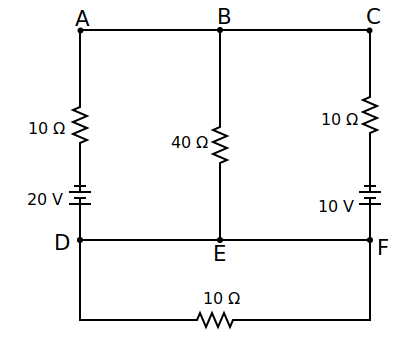
\includegraphics[width=9cm]{fig4}}
	\caption{نمونه یک مدار الکتریکی }
	\label{fig:fig4}
\end{figure}

\begin{figure}[ht]
	\centerline{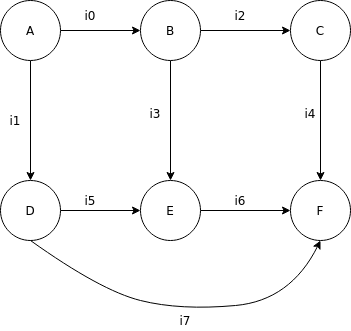
\includegraphics[width=9cm]{fig5}}
	\caption{گراف مدل شده شکل
\ref{fig:fig4}	
}
	\label{fig:fig5}
\end{figure}
پس از مدل کردن مدار به صورت گراف نوبت به یافتن دور های ساده گراف مدل شده میشود،
طبق الگوریتم
\ref{simpcyc}
تمامی دور های ساده گراف را میابیم.
این دور های ساده عبارت اند از
\lr{ABEDA}
،
\lr{BCFEB}
و
\lr{DEFD}
.
این دور های ساده هر یک مشخص کننده یک معادله
\lr{KVL}
هستند
\footnote{
هر دور در گراف مدل شده چه ساده و چه غیرساده بیانگر یک قانون
\lr{kvl}
است ولی قانونی که از یک دور غیرساده بدست می آید به از لحاظ جبری
مستقل از دور های ساده تشکیل دهنده آن نیست.
}
،بدین صورت که مجموع اختلاف پتانسیل های یک دور بایستی برابر صفر شود،
به عنوان نمونه برای دور 
\lr{ABEDA}
داریم :
\begin{equation}\label{eq:kvl_for_ABEDA}
\Delta V_{AB} + \Delta V_{BE} + \Delta V_{ED} + \Delta V_{DA} = 0
\end{equation}
طبق عناصر موجود در هر شاخه میدانیم که
\begin{equation}\label{eq:kwneqs}
	\Delta V_{AB} = 0
	,
	\Delta V_{BE} = -40 I_3
	,
	\Delta V_{ED} = 0 
	,
	\Delta V_{DA} = - 20 + 10 I_1
	\footnote{
دقت کنید که چون در شکل
    \ref{fig:fig5}
    جهت جریان
    \lr{i1}
    از
    \lr{A}
    به
    \lr{D}
    است بدین خاطر علامت به طور کلی
    قرینه شده است.
	}
\end{equation}
با جایگذاری معادله
\ref{eq:kwneqs}
در
\ref{eq:kvl_for_ABEDA}
به این نتیجه میرسیم:
\begin{equation}\label{eq:kvl_for_ABEDA}
	10 I_1 - 40 I_3 = 20
\end{equation}
با تکرار مراحل فوق برای دور های ساده
\lr{BCFEB}
و
\lr{DEFD}
دو معادله 
\lr{kvl}
دیگر پیدا میشود.
این دو معادله، عبارت اند از
 \begin{equation}
	\begin{cases}
		10 I_7 = 0\\
		-40 I_3 + 10 I_4 = + 10
	\end{cases}\,.
\end{equation}
با یافتن تمامی قوانین
\lr{kvl}
نوبت به یافتن قوانین
\lr{kcl}
میرسد، هر راس از گراف بیانگر یک قانون 
\lr{kcl}
است ولی از 
\lr{n}
قانون موجود تنها
\lr{n-1}
قانون از لحاظ جبری مستقل
\footnote{
استقلال جبری یک معادله از چندین معادله دیگر بدین معنی است که معادله یاد شده
یک ترکیب خطی از دیگر معادلات نباشد.
}
اند و قانون
\lr{n}
ام،
جبرا وابسته به
\lr{n-1}
معادله پیشین است.

به عنوان نمونه معادله 
\lr{kcl}
مربوط به راس
\lr{A}
\footnote{ 
	در نظر داشته باشید که طبق شکل
	\ref{fig:fig4}
	جهت جریان 
	\lr{I0}
	و
	\lr{I1}
	اینگونه تعریف شده است،
	این جهت ها ممکن است اشتباه باشد و اگر اینطور باشد جواب بدست آمده منفی خواهد شد معنی آن این است که جریان با همین مقدار در خلاف جهت یاد شده وجود دارد.
}
برابر است با
:
\begin{equation}\label{eq:kvl_for_ABEDA}
		-I_0 -I_1 = 0
\end{equation}

با بدست آوردن معادلات
\lr{kcl}
 مربوط به راس های دیگر حال بایستی اقدام به حل یک دستگاه معادلات بکنیم،
 برای این مثال دستگاه بدین صورت است:
 \begin{equation}
	\begin{cases}
		10 I_1 - 40 I_3 = 20\\
		10 I_7 = 0\\
		-40 I_3 + 10 I_4 = 10\\
		-I_0  -I_1 = 0\\
		I_0 -I_2 -I_3 = 0\\
		+I_2 - I_4 = 0 \\
		+I_1 - I_5 = 0 \\
		+I_3 + I_5 - I_6 = 0
	\end{cases}\,.
\end{equation}
از آنجایی که هر دستگاه معادلات خود یک معادله ماتریسی است پس داریم:
 \begin{equation}
\begin{pmatrix}
	0 & 10 & 0 & -40 & 0 & 0 & 0 & 0\\
	0 & 0 & 0 & 0 & 0 & 0 & 0 & 10\\
	0 & 0 & 0 & -40 & +10 & 0 & 0 & 0\\
	-1 & -1 & 0 & 0 & 0 & 0 & 0 & 0\\
	1 & 0 & -1 & -1 & 0 & 0 & 0 & 0\\
	0 & 0 & 1 & 0 & -1 & 0 & 0 & 0\\
	0 & 1 & 0 & 0 & 0 & -1 & 0 & 0\\
	0 & 0 & 0 & 1 & 0 & 1 & -1 & 0\\
\end{pmatrix}
\times
\begin{pmatrix}
I_0\\
I_1\\
I_2\\
I_3\\
I_4\\
I_5\\
I_6\\
I_7\\
\end{pmatrix}
=
\begin{pmatrix}
	20\\
	0\\
	10\\
	0\\
	0\\
	0\\
	0\\
	0\\
\end{pmatrix}
\end{equation}

با حل معادله فوق نتیجه میشود:
 \begin{equation}
	\begin{pmatrix}
		I_0\\
		I_1\\
		I_2\\
		I_3\\
		I_4\\
		I_5\\
		I_6\\
		I_7\\
	\end{pmatrix}
	=
	\begin{pmatrix}
		-\frac{2}{3}\\
		\frac{2}{3}\\
		-\frac{1}{3}\\
		-\frac{1}{3}\\
		-\frac{1}{3}\\
		\frac{2}{3}\\
		\frac{1}{3}\\
		0\\
	\end{pmatrix}
\end{equation}
بدین گونه جریان هر شاخه پیدا میشود، همانطور که پیشتر یاد شد وجود علامت منفی به این 
معنا است که جریان در خلاف جهت گمان شده وجود دارد.
گراف کیرشهف پس از یافتن جواب را در شکل
\ref{fig:fig6}
 میتوانید مشاهده کنید.
\begin{figure}[ht]
	\centerline{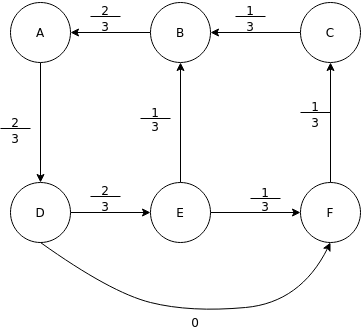
\includegraphics[width=9cm]{fig6}}
	\caption{جواب مدار شکل
		\ref{fig:fig4}	
	}
	\label{fig:fig6}
\end{figure}

\section{حل یک نمونه از مدار
\lr{RC} }

\section{حل یک نمونه از مدار
	\lr{RL} }

\section{جمع بندی}